\documentclass[a4paper,landscape,twocolumn,11pt,gray]{article}

\usepackage{préambule}
\usepackage[export]{adjustbox}

\addtolength{\topmargin}{-1.5cm}
\addtolength{\textheight}{1.5cm}

\title{Utilisation de GeoGebra}
\date{}
\author{}

\begin{document}

\maketitle

\begin{attention}[frametitle={⚠}]
	Si GeoGebra n'est pas présent sur l'ordinateur, utilise la version en ligne à l'adresse \url{https://www.geogebra.org/classic}.
\end{attention}

\section{Se déplacer dans GeoGebra}

\begin{itemize}
	\item Pour bouger sur la grille, tu peux utiliser l'outils \squared{Déplacer} :

	      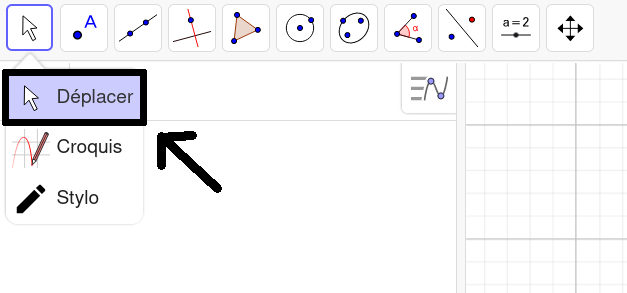
\includegraphics[width=0.3\textwidth,frame]{Images/GeoGebra-Déplacer.png}

	      Cet outils sert également à déplacer les objets créés.
	\item Utilise la molette de la souris pour zoomer/dézoomer.
	\item Pour modifier les propriétés d'un objets, tu peux :

	      \begin{tabular}{p{0.23\textwidth}|p{0.23\textwidth}}
		      Faire click \textbf{droit} sur l'objet :                                 & Utiliser le menu de gauche :                                              \\
		      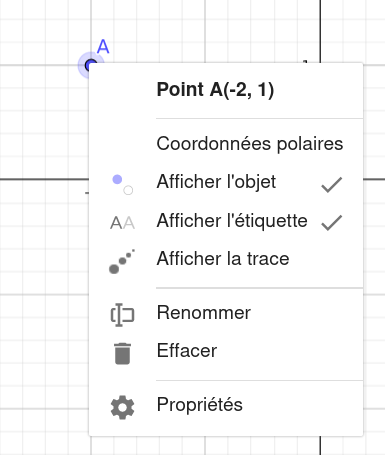
\includegraphics[width=0.125\textwidth,frame]{Images/GeoGebra-click_droit.png} & 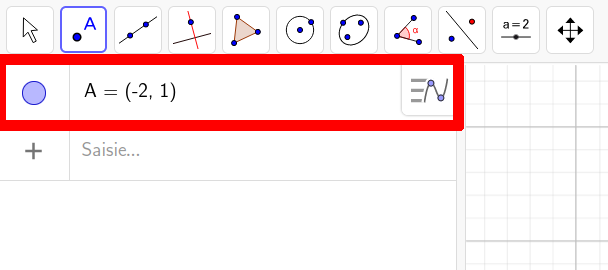
\includegraphics[width=0.2\textwidth,frame]{Images/GeoGebra-Menu_de_gauche.png}
	      \end{tabular}
\end{itemize}

\section{Créer des objets}

Tous les objets se créent via le menu supérieur.


\includegraphics[width=0.4\textwidth,frame]{Images/GeoGebra-Menu_supérieur.png}

\begin{tabular}{p{0.23\textwidth}p{0.23\textwidth}}
	∙ Créer un point :                                                      & ∙ Créer une droite ou un segment :                                              \\
	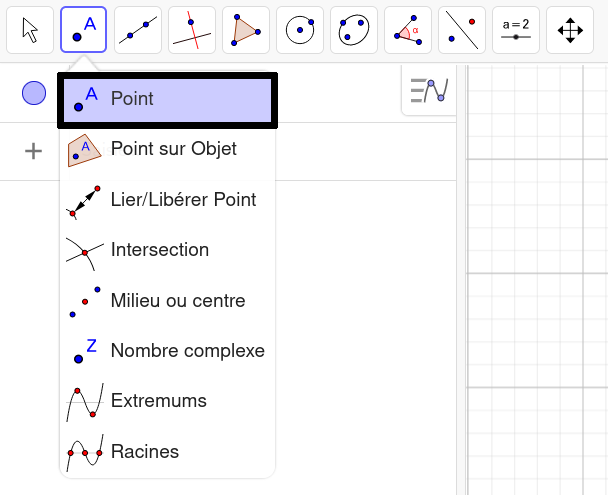
\includegraphics[width=0.22\textwidth,frame]{Images/GeoGebra-Créer_point.png}  & 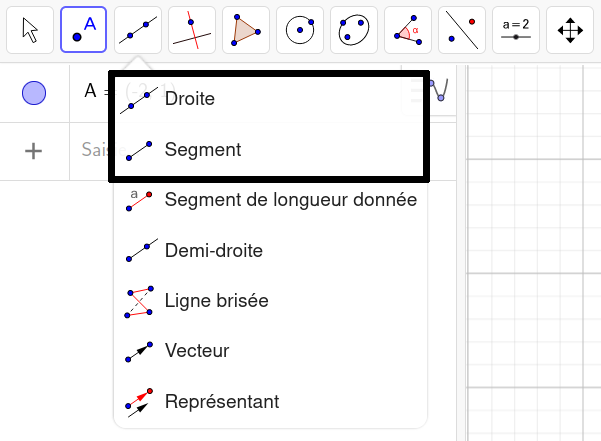
\includegraphics[width=0.22\textwidth,frame]{Images/GeoGebra-Créer_droite_segment.png} \\
	∙ Prendre le milieu d'un segment :                                      & ∙ Faire une symétrie centrale :                                                 \\
	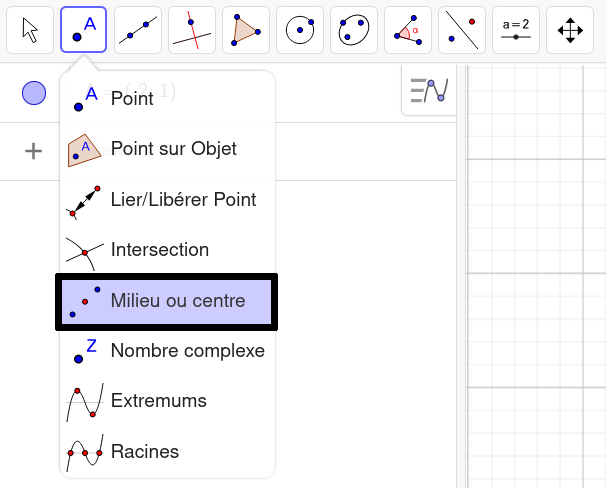
\includegraphics[width=0.22\textwidth,frame]{Images/GeoGebra-Créer_milieu.png} & 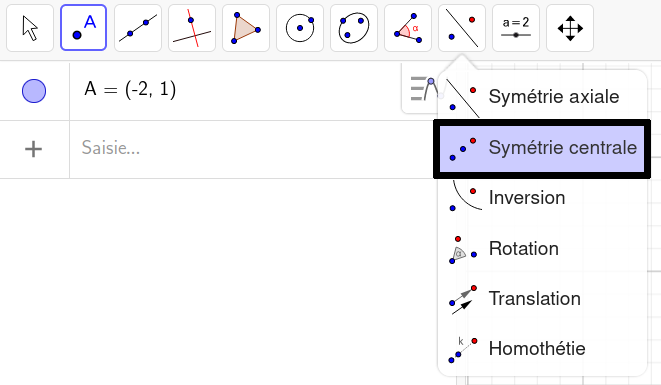
\includegraphics[width=0.22\textwidth,frame]{Images/GeoGebra-symétrie_centrale.png}
\end{tabular}

\end{document}